\documentclass{article}
\usepackage[utf8]{inputenc}
\usepackage{mathtools}
\usepackage{whilecode2}
\usepackage{listings}
\usepackage{fancyhdr}
\usepackage{graphicx}
\usepackage[colorlinks=true, allcolors=blue]{hyperref}
\pagestyle{fancy}
\lhead{Iván López Cervantes}
\rhead{\thepage}
\cfoot{}
\author{Ivan Lopez Cervantes }

\date{}
\begin{document}
\title{Práctica 4}
\maketitle

\section*{Ejercicio 1}
Crea el programa WHILE más simple que compute la función divergente (con cero argumentos) y computa la codificación de su código
\subsection*{Solución}
El código WHILE sería el siguiente:\\
\whileprogram{Q}{0}{
 
}{s}

\begin{whilecode}[H]
\DefaultVar{2}\Assig\DefaultVar{1} + 1\\
 \While{$X_2 \not = 0$}{

  $X_1 \Assig 0$\;
}
\end{whilecode}
Codificación del WHILE:\\
\[
WHILE2N(0, X_2 = X1 + 1;\; while\; X_2 \neq 0\; do\; X1 = 0\;od) = \boxed{59170879}
\]
Desarrollo del cálculo: \\
\begin{gather*}
WHILE2N(0, X_1 = X1 + 1;\; while\; X_1 \neq 0\; do\; X1 = X1\;od) = \sigma^2_1(0, code2N(s))\\
\textbf{Descomponemos code2N(s):}\\
code2N(s) = \Gamma(sent2N(X_2 = X_1 + 1),sent2N( while\; X_2 \neq 0\; do\; X1 = 0\; od)) - 1 = 10876\\
\textbf{Calculamos cada sent2N()}\\
sent2N(X_2 = X_1 + 1) = 5\sigma^2_1(1,0) + 2 = 2\\
sent2N( while\; X_2 \neq 0\; do\; X1 = 0\; od) = 5\sigma^2_1(0,Code2N(X_1 = 0)) + 4 = 5\sigma^2_1(0, 0) + 4 = 4 \\
Code2N(X_1 = 0) = \Gamma(sent2N(X_1=0)) - 1 = 0 \\
sent2N(X_1=0) = 5(0) = 0
\end{gather*}

\section*{Ejercicio 2}
Crea un script de Octave que enumere todos los vectores
\subsection*{Solución}
Código del script de Octave
\begin{lstlisting}[language=Octave]
function printALLvectors()
  i = 0;
  while i>=0
   disp(['(' num2str(godeldecoding(i)) ')' ]);
  i++;
  endwhile
end

\end{lstlisting}
Ejemplo de ejecución: \\
\begin{figure}[h]
    \centering
    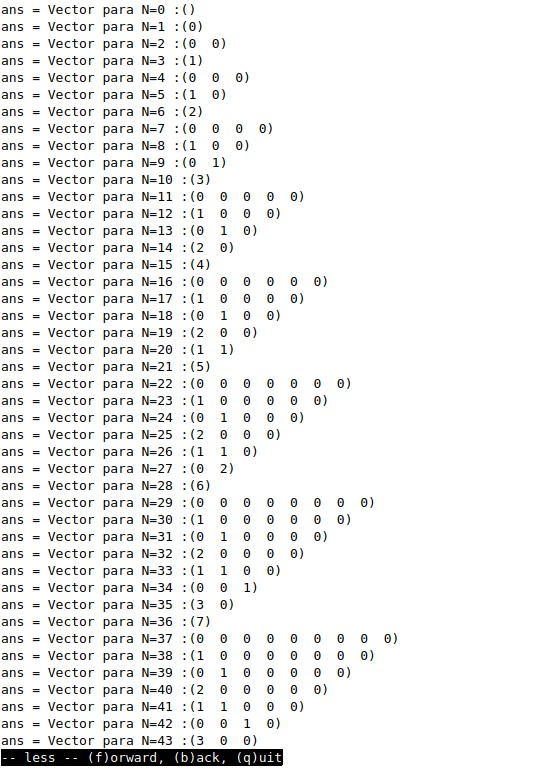
\includegraphics[scale=0.5]{vectores.jpg}
\end{figure}
\section*{Ejercicio 3}
Crea un script de Octave que enumere todos los programas WHILE
\subsection*{Solución}
Código del script de Octave
\begin{lstlisting}[language=Octave]
function printALLWhilePrograms()
  i = 0
  while i>=0
    disp(N2WHILE(i));
    i++;
  endwhile
end

\end{lstlisting}
Ejemplo de ejecución: \\
\begin{figure}[h]
    \centering
    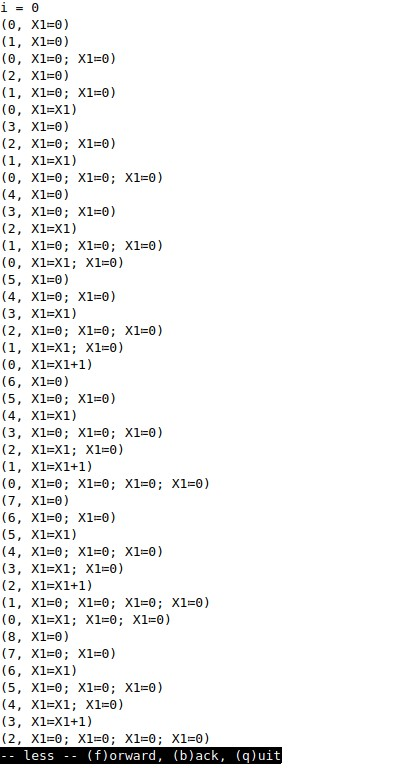
\includegraphics[scale=0.5]{while.jpg}
\end{figure}
\end{document}
